% ======================================
%            Chapter 2A.3
%  Osmosis: A Special Case of Diffusion
%        Created by Michael Tang
%             2025.02.17
% ======================================

\subsubsection{2A.3 Osmosis: A Special Case of Diffusion}
\paragraph{What is Osmosis?}
\begin{itemize}
    \item Osmosis is the movement of free water molecules through a partially permeable membrane from an area of high water
    potential to an area of low water potential.
    \item Water potential is a measure of the potential for water to move in or out of a solution due to osmosis. It depends on
    the concentration of free water molecules.
    \item Water always moves doen the water potential gradient, meaning form areas of high water potential (more free water
    molecules) to low water potential (less free water molecules).
    \item Water moves through membranes, but solute molecules cannot move in the same way.
    \begin{figure}[H]
        \centering
        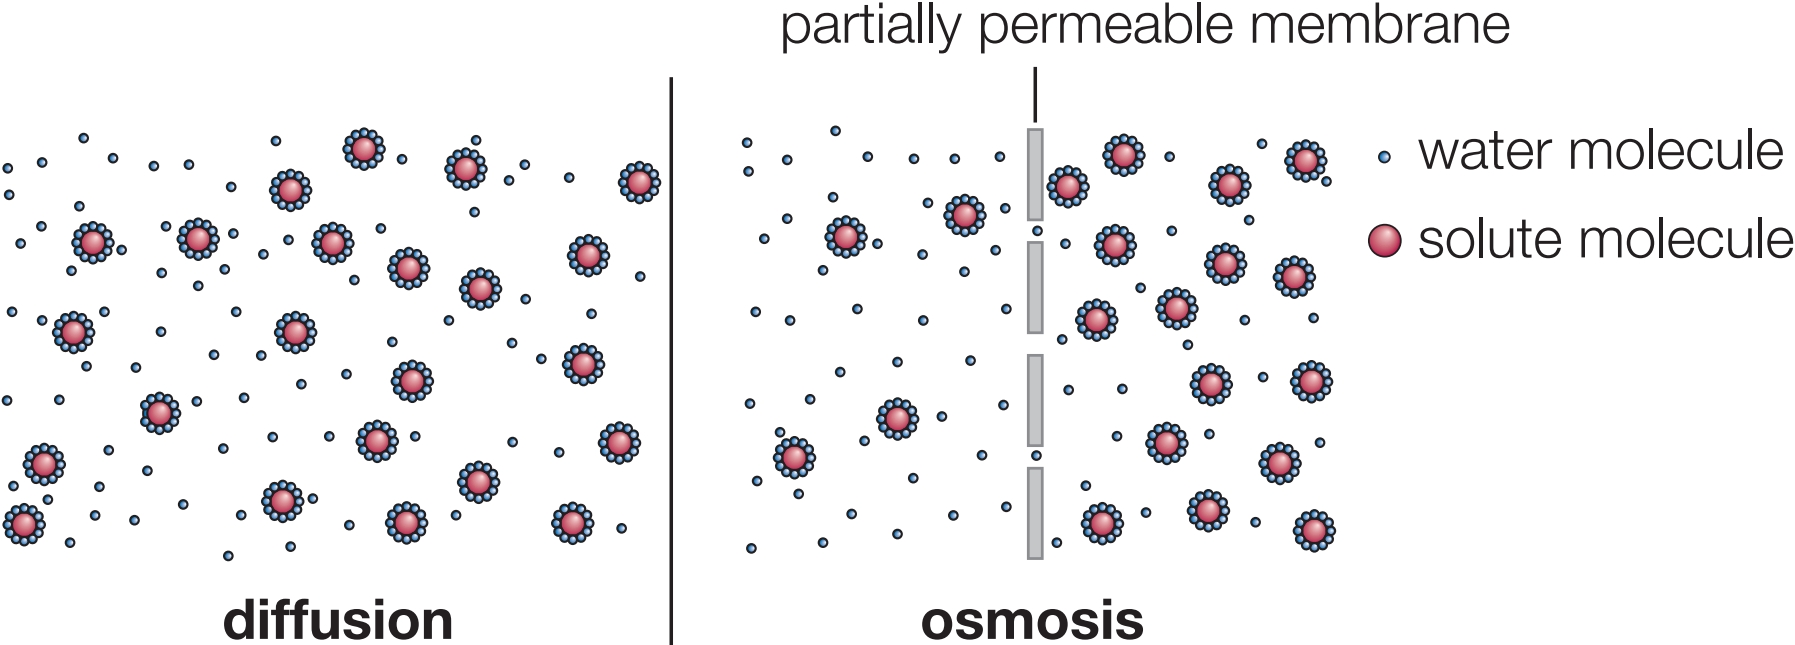
\includegraphics[scale=0.12]{Biology/2A/Images/2A-3-1.png}
        \caption{In diffusion, the random movement of particles results in an even distribution of both solute and solvent
        particles. In osmosis, a partially permeable membrane means only solvent molecules and very small solute particles can
        move freely.}
    \end{figure}
\end{itemize}

\paragraph{Osmotic Concentrations}
\begin{itemize}
    \item Osmotic concentration refers to the amount of dissolved solutes in a solution. A solution with more solutes has lower
    water potential.
    \item Solutions are categorized as:
    \begin{itemize}
        \item \textbf{\underline{Isotonic solution} (等渗溶液):} The concentration of solutes is the same as inside the cell.
        \item \textbf{\underline{Hypotonic solution} (低渗溶液):} The concentration of solutes is lower than inside the cell,
        causing water to enter the cell.
        \item \textbf{\underline{Hyperonic solution} (高渗溶液):} The concentration of solutes is higher than inside the cell,
        causing water to leave the cell.
    \end{itemize}
\end{itemize}

\paragraph{Osmosis in Animal Cells}
Animal cells must maintain a delicate balance of water to prevent cell bursting or shrinking.
\begin{itemize}
    \item \textbf{Hypotonic solution:} Water enters the cell, causing it to swell and burst.
    \item \textbf{Hypertonc solution:} Water leaves the cell, causing it to shrink and shrivel.
\end{itemize}
\begin{figure}[H]
    \centering
    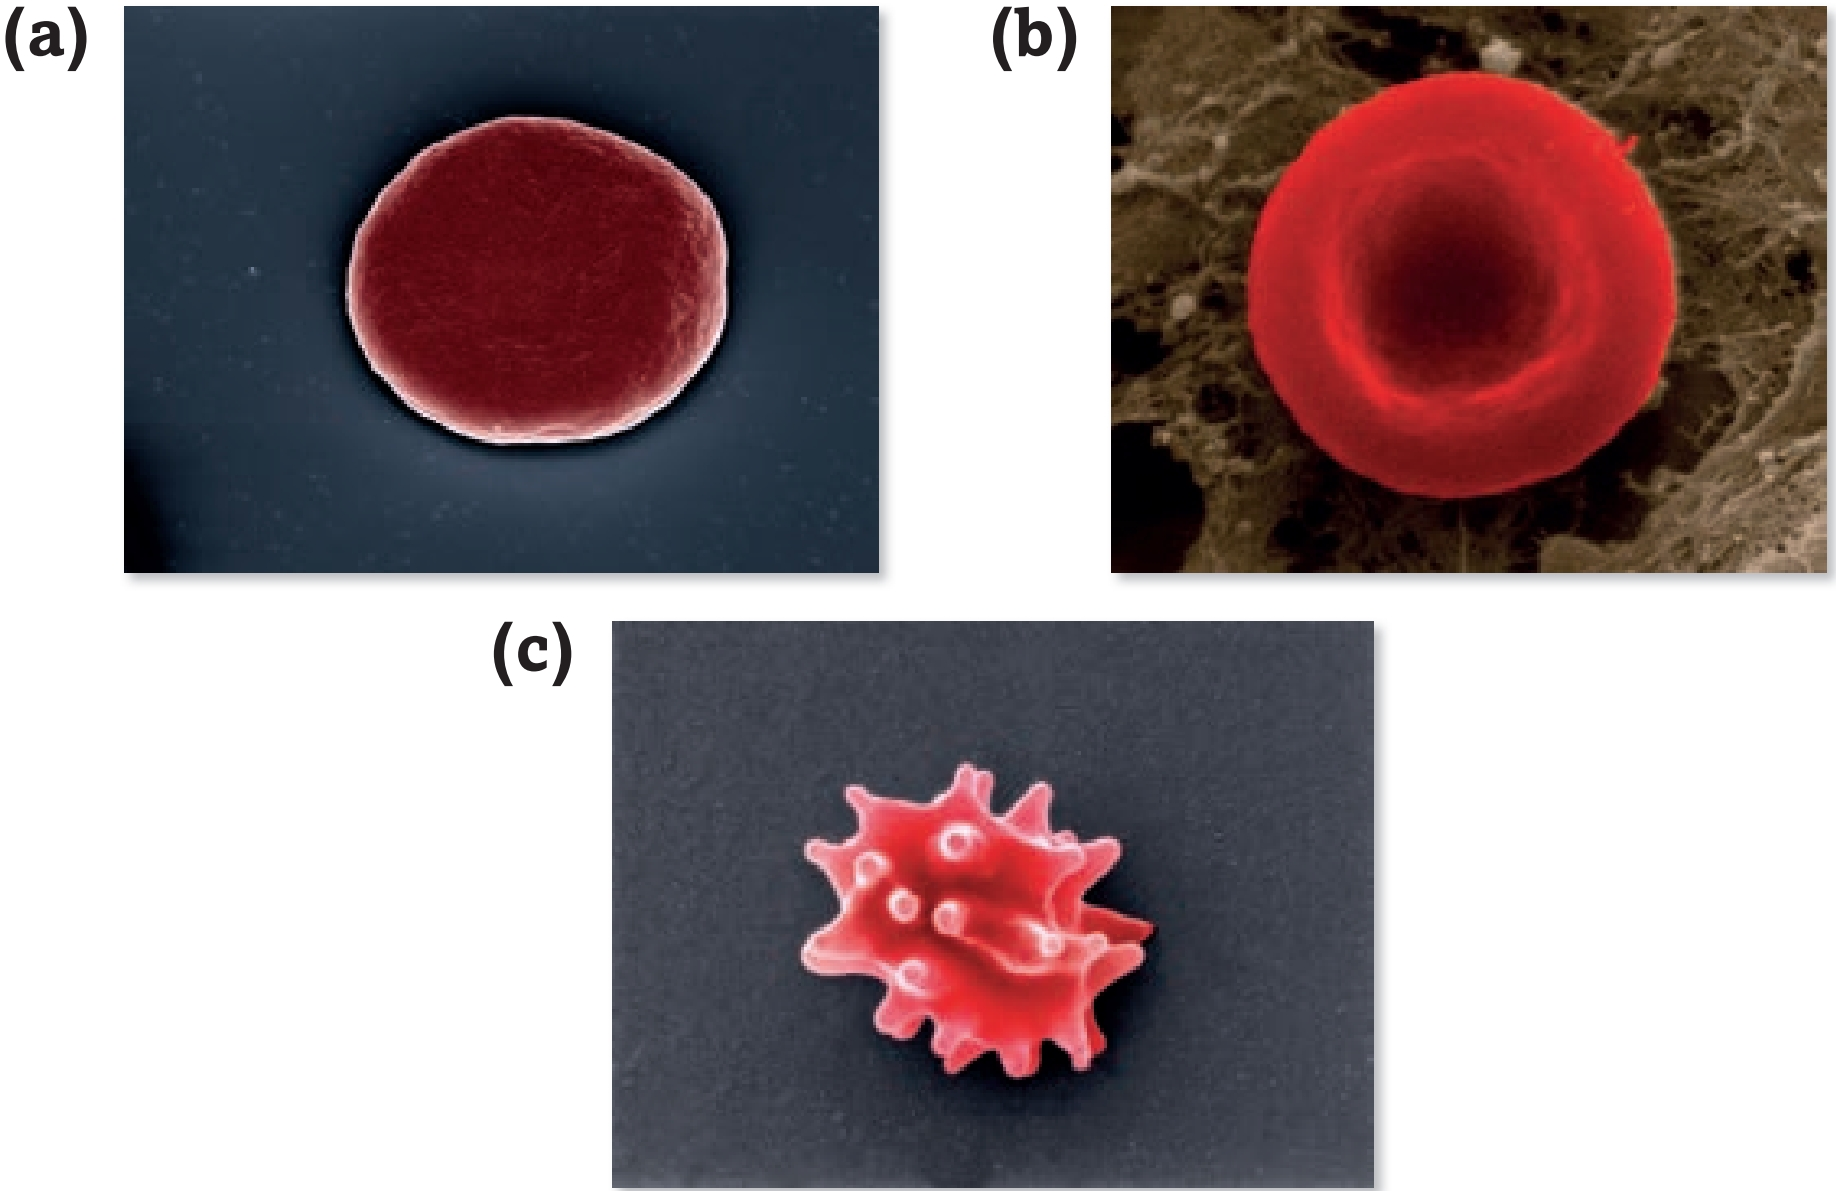
\includegraphics[scale=0.12]{Biology/2A/Images/2A-3-2.png}
    \caption{The effects of osmosis on red blood cells show why the systmes of the body that maintain solute concentrations and
    water balance are so important. \textbf{(a)} In hypotonic solution, water moves in and the cell swells and brusts;
    \textbf{(b)} in isotonic solution the red blood cell maintains its normal shape; \textbf{(c)} in hypertonic solution, water
    moves out and the cell shrinks.}
\end{figure}

\paragraph{Osmosis in Plant Cells}
Plant cells are more resistant to osmotic pressure due to their rigid cell walls.
\begin{itemize}
    \item \textbf{Hypotonic solution:} Water enters the cell, causing it to swell and generate hydrostatic pressure (inward
    pressure that prevents further water influx). This is called \underline{turgor} (膨压).
    \item \textbf{Hypertonic solution:} Water exits the cell, causing the \underline{protoplast} (原生质, cell contents) to
    shrink from the cell wall in a process called \underline{plasmolysis} (胞质裂解).
\end{itemize}
\begin{figure}[H]
    \centering
    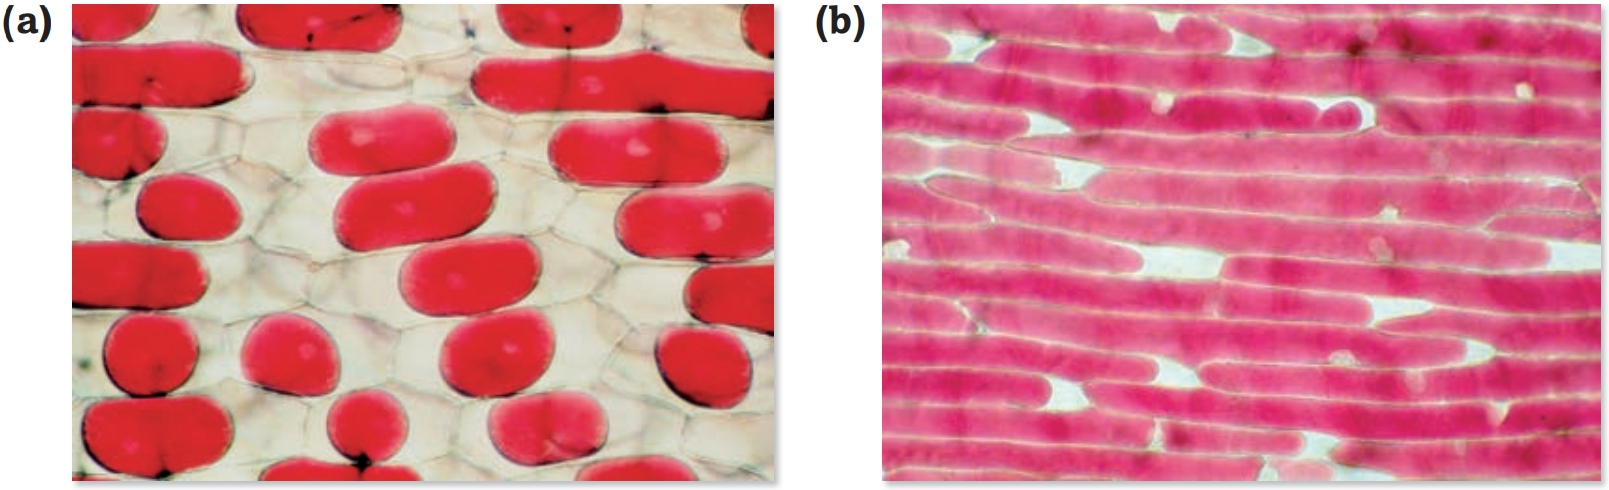
\includegraphics[scale=0.15]{Biology/2A/Images/2A-3-3.png}
    \caption{Plant cells from red beet showing \textbf{(a)} plasmolysis; and \textbf{(b)} turgor.}
\end{figure}

\paragraph{Modelling Osmosis in Cells}
\begin{itemize}
    \item \textbf{Experimental model:} We can model osmosis using an artificial membrane to \underline{demonstrate} (证明) the
    movement of water through a \underline{partially permeable membrane} (半透膜).
    \item \textbf{Sucrose solution} can be used to \underline{illustrate} (说明) osmotic movement (water moves to the area with
    higher solute concentration).
\end{itemize}

\paragraph{Exam Tips}
\begin{itemize}
    \item Use the term water potential to explain osmotic movement in and out of cells.
    \item \textbf{Remember the gradient:} Water always moves from high to low water potential.
    \item Osmosis requires \textbf{no ATP} - It is a passive process relying on kinetic energy of water molecules.
\end{itemize}